\section{Theoretische Grundlagen}
\label{sm_chapter}
In diesem Kapitel wollen wir Ihnen den theoretischen Hintergrund, der f"ur diesen Versuch relevant ist, vermitteln. Dazu fassen wir die relevantesten Aspekte des Standardmodells (SM) der Teilchenphysik, das die fundamentalen Bestandteile und Wechselwirkungen der Natur beschreibt, in Abschnitt \ref{kapsm} zusammen. Eine detaillierte Einf\"uhrung finden Sie in der entsprechenden Fachliteratur \cite{Griffiths, Berger}. Da das Top-Quark in diesem Versuch eine besondere Rolle spielt, wird es in Abschnitt \ref{kaptop} noch einmal gesondert eingef\"uhrt und diskutiert.

% +++++++++++ Standardmodell und Top-Quark +++++++++++++++++
\subsection{Das Standardmodell der Teilchenphysik}
\label{kapsm}
Das Standardmodell der Teilchenphysik bildet den wichtigsten theoretischen Rahmen f\''ur die Ph\''anomene der Teilchenphysik und der gro\ss{}e Erfolg des Modells ist beeindruckend. So wurden viele Vorhersagen des Standardmodels durch zahlreiche Experimente sehr genau best\''atigt. Insbesondere die Entdeckung vorhergesagter Elementarteilchen verdeutlicht dessen M\''achtigkeit. Und dennoch deckt das SM in seiner jetzigen Form nicht alle Beobachtungen ab. So ist unter anderem die Gra\-vi\-ta\-tion nicht im SM enthalten. Des Weiteren gibt es Hinweise auf dunkle Materie und dunkle Energie, die weder direkt durch ein Experiment beobachtet werden konnten, noch durch das SM vorhergesagt sind.
\\
\\
Nach heutigem Wissenstand setzt sich die gesamte sichtbare Materie unseres Universums aus den fundamentalen Teilchen des Standardmodells zusammen. Diese unterteilt man nach ihrem Spin in Fermionen (Spin-$1/2$) und Bosonen (Spin-$1$).\\
Innerhalb der Fermionen unterscheidet man zwischen geladenen ($Q = -1$) und neutralen ($Q = 0$) Leptonen, sowie up-artige ($Q = 2/3$) und down-artige ($Q = -1/3$) Quarks. Abschlie\ss{}end werden die verschiedenen Leptonen und Quarks jeweils nach aufsteigender Masse in Paaren zusammengefasst und bilden die drei Generationen der Elementarteilchen. Zus''atzlich dazu enth\''alt das Standardmodell zu jedem Teilchen ein Antiteilchen mit den selben Eigenschaften, aber umgekehrter Ladung. Eine Auflistung der Fermionen ist in Tabelle \ref{Fermionen} zu finden.
% Tabelle: Fermionen
\begin{table}[tp]
\centering
\begin{tabular}{c|c||ccc}
  \cline{3-5}
   \multicolumn{2}{c|}{\multirow{2}{*}{}} & \multicolumn{3}{c}{Generationen}\\
   \multicolumn{2}{c|}{} & 1. & 2. & 3. \\
  \hline
  \multirow{4}{*}{\rotatebox{90}{Leptonen}} & Neutral ($Q=0$) & $\nu_{e}$ & $\nu_{\mu}$ & $\nu_{\tau}$ \\
   \cline{2-5}
   & Geladen ($Q=-1$) & $e$ & $\mu$ & $\tau$ \\
  \hline \hline
  \multirow{4}{*}{\rotatebox{90}{Quarks}} & up-artig ($Q=+\frac{2}{3}$) & $u$ & $c$ & $t$ \\
  \cline{2-5}
   & down-artig ($Q=-\frac{1}{3}$) & $d$ & $s$ & $b$ \\
  \hline
\end{tabular}
	  	\caption{Fermionen des SM mit ihrer Ladung (Q) und Masse \cite{pdg}. Die Massengrenzen der Neutrinos konnten "uber Experimente mit Neutrinooszillationen ermittelt werden.}
	  		\label{Fermionen}
\end{table}
\\
Die Wechselwirkungen zwischen den Teilchen werden durch die Eichbosonen vermittelt. Dazu geh\''oren das Photon ($\gamma$), die geladenen W-Bosonen ($W^{\pm}$), das neutrale $Z^{0}$-Boson, sowie die 8 Gluonen. Eine \"Ubersicht der Bosonen und deren Eigenschaften findet sich in Tabelle \ref{Eichbosonen}. \\
\\

Die elektromagnetische Wechselwirkung wird durch den Austausch virtueller Photonen vermittelt. Photonen koppeln zu Teilchen mit elektrischer Ladung, sind jedoch selbst elektrisch neutral und k\"onnen folglich nicht mit sich selbst wechselwirken. Die zugrundeliegende Theorie ist die Quantenelektrodynamik (QED), die auf der $U(1)_{Q}$-Sym\-me\-trie\-grup\-pe basiert.\\
\\
Die schwache Wechselwirkung wird \"uber die $W^{\pm}$- und $Z^{0}$-Bosonen \"ubertragen. Diese vermitteln zwischen den Fermionen mit schwachem Isospin $T_{3}$. Durch die hohen Massen der W-Bosonen von $m_{W} = 80,4\,\mathrm{GeV/c^{2}}$ und der Z-Masse von $m_{Z} = 91,2\,\mathrm{GeV/c^{2}}$ ist die Reichweite der Wechselwirkung sehr gering. Im Bestreben die Kr\''afte des Standardmodells zu Vereinheitlichen gelang es die elektromagnetische und schwache Wechselwirkung miteinander zu verkn\''upfen. Es resultiert die elektroschwache Theorie, die auf der $SU(2)_{L}\times SU(1)_{Y}$-Symmetrie beruht. Die Quantenzahl $Y = 2(Q - T_{3})$ ist dabei die Hyperladung.\\
Ein wichtiges Ph\''anomen der elektroschwachen Wechselwirkung ist die M\''oglichkeit der Quarks durch Kopplung an ein W-Boson nicht nur in ein Quark der selben Generation, sondern auch anderer Generationen \"uberzugehen. Jedes Quark tr\"agt eine sogenannte \textit{Flavour}-Quantenzahl mit sich, weshalb man auch von Flavour-\"andernden geladenen Str\"omen spricht. Die \"Ubergangswahrscheinlichkeit eines Quark-Flavours zu einem anderen wird \"uber die Ca\-bibbo-\-Ko\-ba\-ya\-shi-\-Maska\-wa\-(CKM)-\-Matrix beschrieben, die wie folgt lautet \cite{pdg}:
\begin{equation}
\textbf{V}_{CKM}=\begin{pmatrix} V_{ud} & V_{us} & V_{ub} \\ V_{cd} & V_{cs} & V_{cb} \\ V_{td} & V_{ts} & V_{tb} \end{pmatrix}=\begin{pmatrix} 0,974 & 0,225 & 0,004 \\ 0,225 & 0,973 & 0,041 \\ 0,009 & 0,040 & 0,999 \end{pmatrix}
\label{CKMmatrix}
\end{equation}
\\
F\"ur geladenen Leptonen wurde bisher kein solcher \"Ubertritt der Generationen beobachtet. Jedoch konnte in den letzten Jahren mit Hilfe verschiedener gro\ss{}er Neutrino-Experimente die Neutrinooszillation nachgewiesen werden. Der oszillierende \"Ubergang der Neutrinos in den drei Generationen ist der entscheidende Hinweis darauf, dass Neutrinos eine Masse besitzen.  
\\
Masselose Gluonen stellen die Austauschteilchen der starken Wechselwirkung dar. Sie koppeln an die \textit{Farbladung}, die in den Zust\"anden blau, rot und gr\"un sowie den entsprechenden Anti-Zust\"anden auftreten. Die zugrundeliegende Theorie ist die Quantenchromodynamik (QCD) mit ihrer Symmetriegruppe $SU(3)_{C}$\footnote{$C$ steht f\"ur \textit{colour} und meint in diesen Zusammenhang die Farbzust\"ande der starken Wechselwirkung.}. Aus der Gruppe der Leptonen tragen lediglich Quarks Farbladung. Dar\"uber hinaus tr\"agt das Gluon selbst Farbladung mit sich, sodass eine Selbstwechselwirkung unter Gluonen m\"oglich ist. Können somit bei hohen Energien und damit kleinen Abst\"anden der Quarks und Gluonen noch als quasi-freie Teilchen behandelt werden, ist dies mit anwachsendem Abschand nicht mehr möglich. Kommt es in Folge einer Teilchenkollision zur Separierung von Quarks und Gluonen wächst der einzige freie Parameter ($\alpha_{s}$) und die Energie des Farbfeldes stetig an. Sie steigt solange an, bis es energetisch g\"unstiger ist ein neues Quark-Antiquark Paar zu bilden. Dies wiederholt sich so lange, bis die Energie des Feldes nicht mehr ausreicht um ein neues Paar zu bilden. Diesen Prozess bezeichnet man als Hadronisierung und den entsehenden kollimierten Teilchenschauer als Jet. 
\\
\begin{table}[tp]
\centering
\begin{tabular}{c||c|c|c}
Eichboson & Masse\,[GeV] & Wechselwirkung & Materieteilchen \\ \hline\hline
8 Gluonen & 0 & stark & Quarks \\ \hline
\multirow{2}{*}{$W^{\pm}$- und $Z^{0}$-Bosonen} & $m_{W}=80,4$ & schwach, & \multirow{2}{*}{Quarks, Leptonen} \\
 & $m_{Z}=91,2$ & elektromagnetisch & \\ \hline
Photon & 0 & elektromagnetisch & Quarks, geladene Leptonen\\ \hline
\end{tabular}
	  	\caption{Die Eichbosonen des SM mit ihren Massen, Wechselwirkungen und Materie\-teilchen, an denen sie koppeln. Die Masse des Gluons ist indes ein theo\-re\-tischer Wert.}
	  		\label{Eichbosonen}
\end{table}


% ======================
% ++++++Top Quark+++++++
% ======================
\subsection{Physik des Top-Quarks}
\label{kaptop}
Seit seiner Entdeckung im Jahr 1995 am Proton-Antiproton-Beschleuniger Tevatron, spielt das Top-Quark eine bedeutende Rolle in der Teilchenphysik. Das liegt insbesondere daran, dass es mit einer Masse von $m_{t}=173,34\pm 0,76$\,GeV \cite{ATLAS:2014wva} das Schwerste aller Quarks ist.\\
W\"ahrend am Tevatron Top-Quarks bei einer Schwerpunkts\-energie von $\sqrt{s}=1,96$\,TeV\footnote{Bei der Entdeckung des Top-Quarks entsprach die Schwerpunkts\-energie am Tevatron $\sqrt{s}=1,8$\,TeV. Erst 2001 wurde die Schwerpunkts\-energie auf 1,96\,TeV erh"oht.} erzeugt wurden, ist seit 2010 eine Produktion bei 7\,TeV bzw. 8\,TeV durch den Large Hadron Collider (LHC) m\"oglich. Bereits 2011 wurden über 800\,000 Top-Quark-Paare am LHC erzeugt, was die M\"oglichkeit offenbart, die Eigenschaften des Top-Quarks sehr pr\"azise zu untersuchen. Dar\"uber hinaus erm\"oglicht es zahlreiche Suchen nach neuer Physik jenseits des Standardmodells, bei der Top-Quarks eine wichtige Rolle spielen.\\
Im Folgenden geht es um die Erzeugung von Top-Quark-Paaren sowie um den Zerfall des Top-Quarks -- vorrangig unter den Vorraussetzungen des LHC -- und dar\"uber hinaus um das Top-Quark jenseits des SM. Ein umfangreicher \"Uberblick zur Physik des Top-Quarks kann in \cite{Bernreuther, Schilling} gefunden werden.


% ======================
% +++ttbar Produktion+++
% ======================
\subsubsection{Top-Quark-Produktion am LHC}
%\footnotetext{\textbf{I}nitial \textbf{S}tate \textbf{R}adiation: Abstrahlung eines Teilchens im Anfangszustand. Die Abstrahlung eines Teilchens im Endzustand wird entsprechend als \textbf{F}inal \textbf{S}tate \textbf{R}adiation bezeichnet.}
\begin{figure}[t]
	\centering
	\includegraphics[scale=0.80]{Theorie/toppairfeynman.eps}
	\caption[Feynman-Diagramme zur $t\overline{t}$-Produktion in verschiedenen Kan"alen]{Feynman-Diagramme zur $t\overline{t}$-Produktion in verschiedenen Kan"alen. In den ersten beiden Reihen wird die $t\overline{t}$-Produktion in f"uhrender Ordnung gezeigt. In der dritten Reihe ist, aufgrund der ISR bzw. $g$-Schleife, die $t\overline{t}$-Produktion in der n"achst-f"uhrenden Ordnung zu sehen.}
	\label{toppairproduction}
\end{figure}
\begin{figure}[t!]
	\centering
	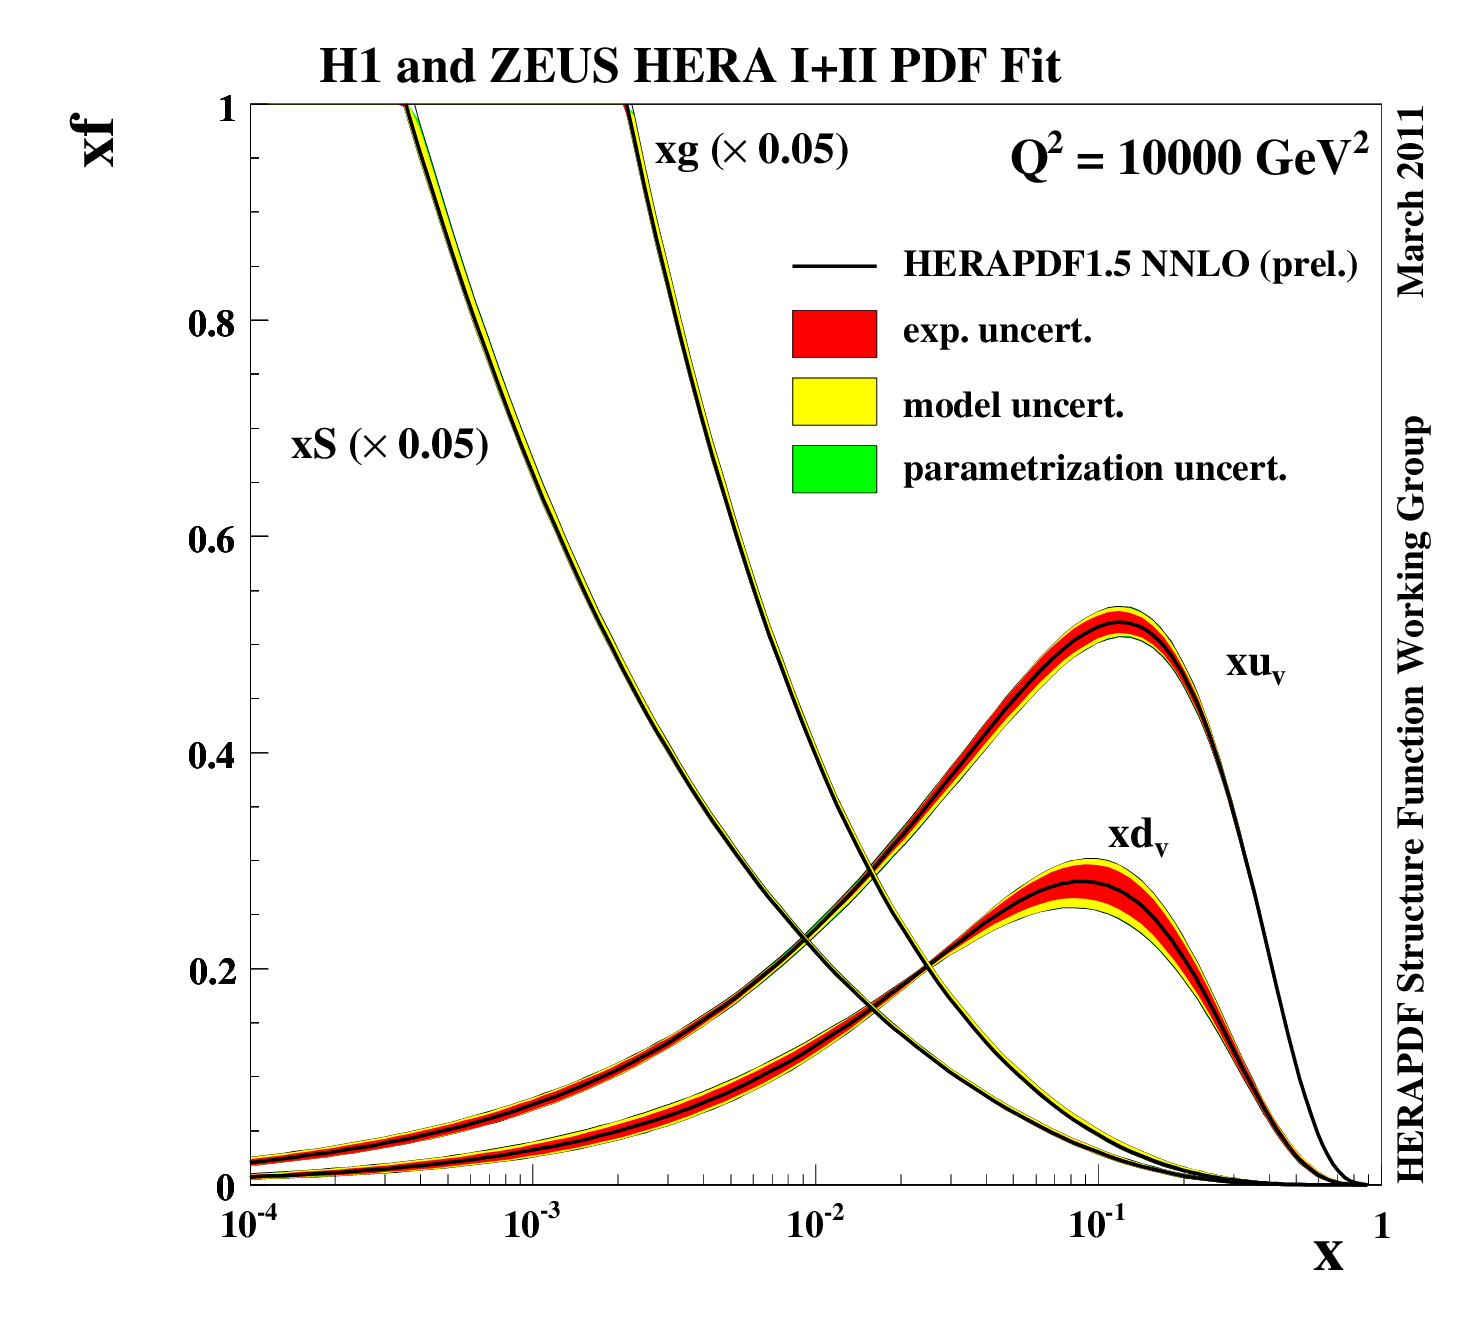
\includegraphics[scale=0.30]{Theorie/herapdf2.png}
	\caption[Parton-Dichte-Funktionen (PDFs) des Protons als Funktion des Impulsbruchteils $x$]{Parton-Dichte-Funktionen (PDFs) des Protons als Funktion des Impulsbruchteils $x$. F"ur einen Viererimpuls"ubertrag von $Q^{2}=10000$\,GeV$^{2}$ sind die PDFs der Valenzquarks ($u_{v},d_{v}$), Seequarks (S) und Gluonen (g) abgebildet \cite{combinedhera}.}
	\label{herannlo}
\end{figure}
Die Produktion von Top-Quark-Paaren im SM wird haupts\"achlich \"uber die starke Wechselwirkung vermittelt. Top-Quark-Paare k\"onnen sowohl in Quark-Antiquark-Annihilationen als auch in Gluon-Gluon-Fusionen produziert werden. Abbildung \ref{toppairproduction} veranschaulicht diese Prozesse. Zur Erzeugung eines $t\overline{t}$-Paares muss die Schwerpunkts\-energie der wechselwirkenden Partonen $\hat{s}$ mindestens der doppelten Top-Quark-Masse ($\approx$350\,GeV) entsprechen. Aus diesem Grund m\"ussen Partonen, unter der Annahme von $x_{1}=x_{2}$, den Impulsbruchteil
\begin{equation}
x_{1,2}\geq \frac{350\,\text{GeV}}{1,96\,\text{TeV}}\approx 0,2 \text{ (Tevatron)},\,\,x_{1,2}\geq \frac{350\,\text{GeV}}{8\,\text{TeV}}\approx 0,04 \text{ (LHC)}
\end{equation}
besitzen, um $t\overline{t}$-Paare erzeugen zu k\"onnen. Abbildung \ref{herannlo} ist zu entnehmen, dass die Valenz\-quarks bei einem Impulsbruchteil von 0,02 in den PDFs dominant sind. Deshalb \"uberwiegt die Quark-Antiquark-Annihilation zur $t\overline{t}$-Paar-Produktion am Tevatron zu ei\-nem Anteil von ungef"ahr 85\,\%. Am LHC liegt ein \"ahnlicher Anteil zugunsten der Gluon-Gluon-Fusion vor. Die dortige Schwerpunkts\-energie von 8\,TeV erlaubt zur $t\overline{t}$-Produktion kleinere Impulsbruchteile, bei denen die Gluondichten steil ansteigen.
\\
\\
Am LHC wird bei einer Schwerpunkts\-energie $\sqrt{s}=8$\,TeV ein inklusiver $t\overline{t}$-Wirkungs\-querschnitt von $229_{-26}^{+24}$\,pb in NLO \cite{Cacciari:2011hy} und $246_{-11}^{+9}$\,pb in NNLO vorhergesagt \cite{Czakon:2013goa}. In Abbildung \ref{ttprodcross} ist der $t\overline{t}$-Produktionswirkungsquerschnitt in gen"aherter NNLO-Pr"azision eingezeichnet. Die Messwerte bei $\sqrt{s}=1,96$\,TeV mit dem D0- und CDF-Experiment sowie bei $\sqrt{s}=7$\,TeV und $\sqrt{s}=8$\,TeV mit dem CMS-Experiment stimmen gut mit der Vorhersage "uberein.\\
\\
%F"ur die Beschreibung der $t\overline{t}$-Signalereignisse werden in dieser Arbeit die Monte-Carlo-Ereignisgeneratoren \Powheg und \Madgraph verwendet. In der Generierung der Ereignisse liegen zwischen \Powheg und \Madgraph dadurch Unterschiede vor, dass Matrixelemente, Teilchenschauer, Hadronisations- oder Pile-Up-Effekte verschieden berechnet werden. So berechnet beispielsweise \Powheg 2$\rightarrow$2 Matrixelemente in NLO, w"ahrend von \Madgraph 2$\rightarrow$n Prozesse simuliert werden k"onnen, wobei $n\leq 9$ ist. \\ \\
Zus\"atzlich zu der $t\overline{t}$-Produktion k\"onnen \"uber die schwache Wechselwirkung einzelne Top-Quarks erzeugt werden. Die Produktionskan\"ale in niedrigster Ordnung sind Abbildung \ref{singletopprod} zu entnehmen. Der $t$-Kanal, bei dem das Top-Quark \"uber die Fusion eines $W$-Bosons und eines $b$-Quarks erzeugt wird, ist dabei der dominante Prozess. Der inklusive Wirkungsquerschnitt des $t$-Kanals betr\"agt 87,2\,pb am LHC bei einer Schwerpunktsenergie von 8\,TeV. Da $u$-Quarks die dominanten Valenzquarks in den PDFs bei $pp$-Beschleunigern sind, ist die Top-Quark-Produktion im $t$-Kanal ladungsasymmetrisch. Es hat des Weiteren zur Folge, dass die Produktion von Top-Quarks (56,4\,pb) der Produktion von Antitop-Quarks (30,7\,pb) mit einem Verh\"altnis von ungef\"ahr 2:1 \"uberwiegt. Im $s$-Kanal liegt mit dem Zerfall in ein Top und ein Antibottom (3,79\,pb) und deren Antiteilchen (1,76\,pb) der analoge Sachverhalt vor.\\
Die assoziierte Produktion ($tW$-Kanal) einzelner Top-Quarks ist ladungssymmetrisch, weil im Anfangszustand ein Gluon und ein (Anti)b-Quark enthalten ist. F\"ur beide Zust\"ande betr\"agt der vorhergesagte Wirkungsquerschnitt 11,1\,pb \cite{Kidonakis:1449411}.

\begin{figure}[ht]
	\centering
	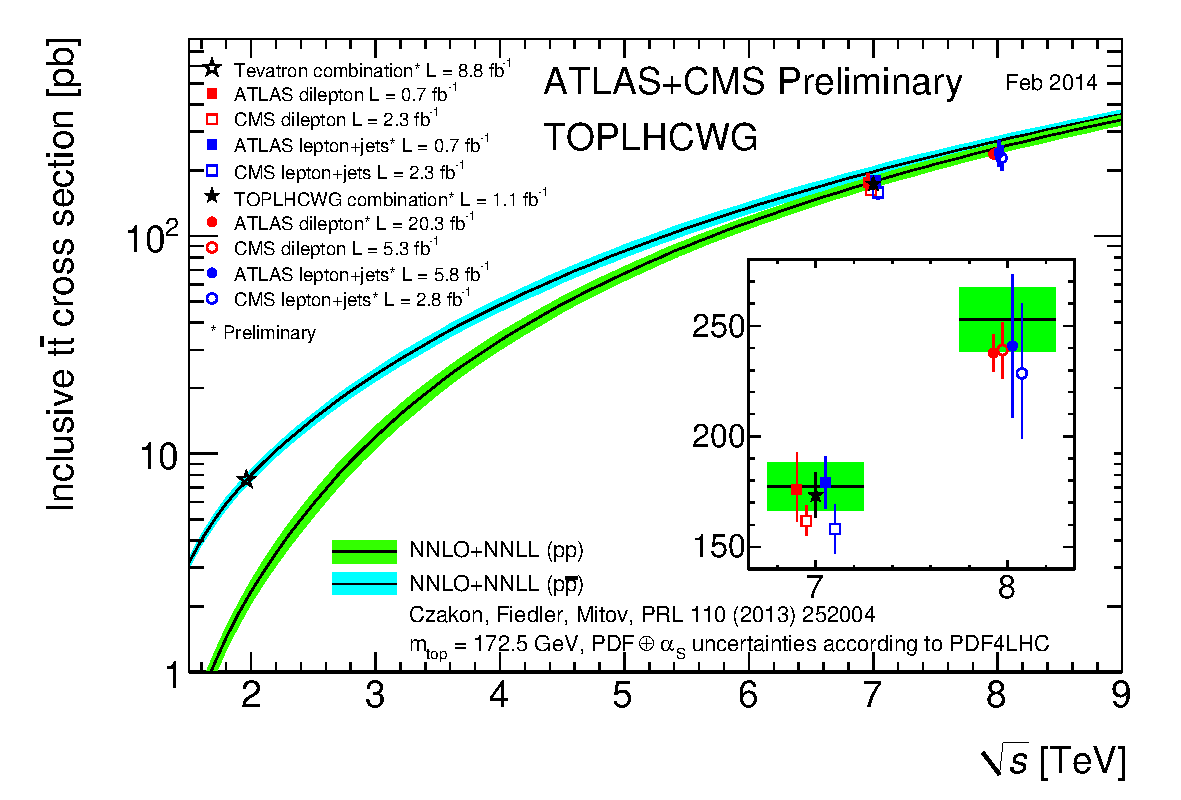
\includegraphics[scale=0.70]{Theorie/ttproductioncrosssection_new.pdf}
	\caption[Der $t\overline{t}$-Produktionswirkungsquerschnitt in Abh\"angigkeit der Schwer\-punkts\-energie]{Der $t\overline{t}$-Produktionswirkungsquerschnitt in Abh\"angigkeit der Schwer\-punkts\-energie. Eingezeichnet sind die Messungen am Tevatron bei $\sqrt{s}=1,96$\,TeV, sowie die Messungen des CMS- und ATLAS-Experiments am LHC bei 7\,TeV und 8\,TeV in verschiedenen Zerfallskan\"alen \cite{prodcrosssectionatlascms}.}
	\label{ttprodcross}
\end{figure}

\begin{figure}[ht]
	\centering
	\includegraphics[scale=0.80]{Theorie/singletopfeynman.eps}
	\caption[Feynman-Diagramme zur Produktion einzelner Top-Quarks in f\"uhrender Ordnung]{Feynman-Diagramme zur Produktion einzelner Top-Quarks in f\"uhrender Ordnung.}
	\label{singletopprod}
\end{figure}



%++++++++++++++++++++++++++++++++++++++++++++++++++++++++
%\footcite{textbf{I}nitial \textbf{S}tate \textbf{R}adiation: Abstrahlung eines Partons im Anfangszustand. Bei Abstrahlungen im Endzustand spricht man entsprechend von textbf{F}inal \textbf{S}tate \textbf{R}adiation}

\subsubsection{Masse und Zerfall des Top-Quarks}
\label{massanddecaytop}
Die Polmasse des Top-Quarks ist ein fundamentaler Parameter des SM. Direkte Messungen am Tevatron ergeben einen Wert von $m_{t}=173,2\pm 0,9$\,GeV \cite{Lancaster:2011wr}. Mit einer Unsicherheit von 0,5\,\% ist die Top-Quark-Masse damit sehr pr\"azise vermessen.
\\
\\
Das Top-Quark kann im SM ausschlie\ss{}lich in ein down-artiges Quark und ein $W$-Boson zerfallen. Die jeweilige Zerfallsrate ist proportional zum Quadrat der Elemente der CKM-Matrix $|V_{tq}|^{2}$ ($q=d,s,b$), sodass der Zerfall in ein W-Boson und ein $b$-Quark mit ca. 99,9\% dominiert (vgl. Gleichung (\ref{CKMmatrix})). Die totale Zerfallsbreite $\Gamma_{t}$ des Top-Quarks im SM ist $\Gamma_{t}=1,33\,\text{GeV} $ \cite{Jezabek:1988iv}. Die gro\ss{}e Zerfallsbreite des Top-Quarks hat eine sehr kurze Lebensdauer von $\tau_{t}=\frac{1}{\Gamma_{t}}\approx 5\cdot 10^{-25}$\,s zur Folge. Die Zeitskala, die Quarks zur Hadronisierung ben\"otigen, liegt in der Gr\"o\ss{}enordnung $\tau_{\text{had}}\sim 10^{-24}$\,s. Top-Quarks zerfallen demzufolge bevor sie hadronisieren k\"onnen, sodass keine gebundenen $t\overline{t}$-Zust\"ande (\textit{Toponium}) existieren.\\
\\
Entsprechend des Zerfalls eines Top-Quarks hat der Zerfall eines $t\overline{t}$-Paares, $t\overline{t}\rightarrow b\overline{b}W^{+}W^{-}$, zwei W-Bosonen und b-Quarks im Endzustand. Die W-Bosonen zerfallen anschlie\ss{}end entweder in ein geladenes Lepton und das zugeh\"orige Neutrino oder in ein $q\overline{q}$-Paar. Der Zerfall in Quark-Paare, die Top-Quarks enthalten, ist aus kinematschen Gr\"unden verboten, da die Masse des Top-Quarks die Masse des W-Bosons \"ubersteigt. Der Zerfall des W-Bosons l\"asst somit drei Zerfallskan\"ale f\"ur den $t\overline{t}$-Zerfall zu, die in Abbildung \ref{leadingorderttbar} dargestellt sind. Die Verzweigungsverh\"altnisse der $t\overline{t}$-Zerfallskan\"ale sind in Tabelle \ref{TopZerfallsraten} zu finden.  \\
\begin{figure}[ht]
	\centering
	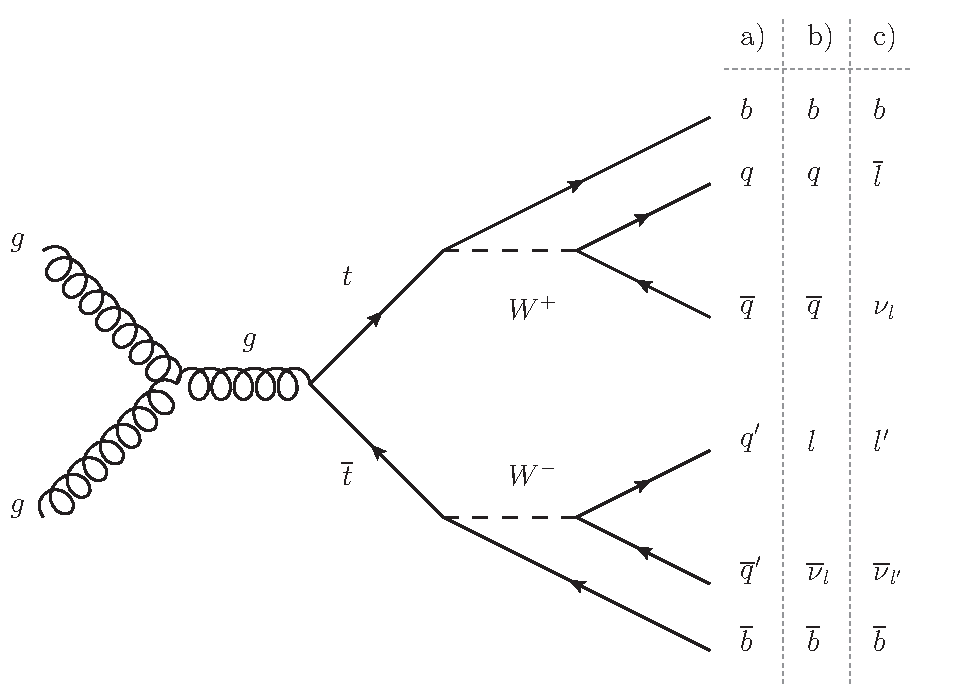
\includegraphics[scale=0.80]{Theorie/leadingorderttproduction-eps-converted-to}
	\caption[Feynman-Diagramm zur $t\overline{t}$-Produktion in f"uhrender Ordnung durch $gg$-Fusion]{Feynman-Diagramm zur $t\overline{t}$-Produktion in f\"uhrender Ordnung durch $gg$-Fusion. Gezeigt ist au"sserdem der weitere Zerfall im voll hadronischen\,(a)), semi\-lep\-tonischen\,(b)) und dileptonischen\,(c)) Kanal.}
	\label{leadingorderttbar}
\end{figure}

\subsubsection*{Voll hadronischer Kanal}
Die gr\"o\ss{}te Zerfallsrate mit 45,7\,\% liegt vor, wenn beide $W$-Bosonen hadronisch zerfallen:
\begin{equation*}
t\overline{t}\rightarrow b\overline{b}W^{+}W^{-}\rightarrow b\overline{b}q\overline{q}'q''\overline{q}'''
\end{equation*}
Neben der gro\ss{}en Zerfallsrate hat dieser Kanal den Vorteil, dass alle Teilchen im Endzustand (zumindest prinzipiell) gemessen werden k\"onnen. Dem entgegen steht ein sehr gro\ss{}er hadronischer Untergrund, der die Rekonstruktion von Quarks zum entsprechenden $t\overline{t}$-Ereignis erschwert.

\subsubsection*{Semileptonischer Kanal}

Die zweitgr\"o\ss{}te Rate (43,8\,\%) f\"ur einen Endzustand liegt vor, wenn eines der $W$-Bosonen hadronisch und das andere leptonisch zerf\"allt:
\begin{equation*}
t\overline{t}\rightarrow b\overline{b}W^{+}W^{-}\rightarrow b\overline{b}q\overline{q}'l\overline{\nu}_{l}
\end{equation*}
In der Praxis wird der semileptonische Kanal auf ein Elektron oder Myon im Endzustand beschr\"ankt, weil das $\tau$-Lepton weiter in Neutrinos und Hadronen bzw. Myonen und Elektronen zerf\"allt, ehe es detektiert werden kann\footnote{Prozesse, bei denen das $\tau$-Lepton in ein Myon oder Elektron zerf\"allt werden jedoch mit ber\"ucksichtigt.}. Die Zerfallsrate f\"ur diesen Kanal reduziert sich damit auf 29,8\,\%. Dessen ungeachtet vereint der semileptonische Zerfalls\-kanal die Vorteile einer gro\ss{}en Zerfallsrate und eines \"uberschaubaren Untergrundes. Die Hauptuntergrundquellen sind W- und Z-Bosonen in Verbindung mit Jets (sogenannte \textit{W-} bzw. \textit{Z-Jets}), einzelne Top-Quarks sowie QCD-Ereignisse. Des Weiteren wird die Rekonstruktion eines $t\overline{t}$-Ereignisses dadurch erschwert, dass das Neutrino nicht detektiert wird. \\
F\"ur diesen Praktikumsversuch wird der semileptonische $t\overline{t}$-Zerfallskan\"al mit einem My\-on (Myon+ Jets-Kanal) im Endzustand betrachtet.

\subsubsection*{Dileptonischer Kanal}
Der dileptonische Zerfallskanal hat mit 10,5\,\% die kleinste Zerfallsrate. Beide $W$-Bosonen zerfallen leptonisch, sodass zwei verschieden geladene Leptonen sowie zwei Neutrinos im Endzustand vorliegen:
\begin{equation*}
t\overline{t}\rightarrow b\overline{b}W^{+}W^{-}\rightarrow l\overline{\nu}_{l}\overline{l}'\nu_{l'}
\end{equation*}
Da die geladenen Leptonen verh\"altnism\"a\ss{}ig leicht vom Untergrund unterschieden werden k\"onnen, hat der dileptonische Zerfallskanal die reinste Signatur. Aufgrund der fehlenden Energie der beiden Neutrinos jedoch, kann die Struktur des $t\overline{t}$-Ereignisses nur sehr schwer rekonstruiert werden. Des Weiteren besteht die bereits f\"ur den semileptonischen Zerfalls\-kanal beschriebene Problematik, dass es sich bei einem geladenen Lepton oder beiden geladenen Leptonen um ein $\tau$-Lepton bzw. zwei $\tau$-Leptonen handelt. Schlie\ss{}t man $\tau$-Leptonen im Endzustand aus, reduziert sich die Zerfallsrate auf 4,6\,\%.


\begin{table}[ht]
\centering
\begin{tabular}{lc|lc}
Kanal & Rate\,[\%] & Kanal & Rate\,[\%] \\ \hline\hline
Dileptonisch & 10,50 $\pm$ 0,12 & $ee$ & 1,16 $\pm$ 0,02 \\
 &  & $\mu\mu$ & 1,12 $\pm$ 0,02 \\ 
 &  & $\tau\tau$ & 1,27 $\pm$ 0,03 \\
 &  & $e\mu$ & 2,27 $\pm$ 0,04 \\ 
 &  & $e\tau$ & 2,42 $\pm$ 0,05 \\
 &  & $\mu\tau$ & 2,38 $\pm$ 0,05 \\ \hline
Semileptonisch & 43,80 $\pm$ 0,40 & $e$+Hadronen & 14,53 $\pm$ 0,19 \\
 & & $\mu$+Hadronen & 14,29 $\pm$ 0,21 \\
 & & $\tau$+Hadronen & 15,21 $\pm$ 0,28 \\ \hline
Voll hadronisch & 45,70 $\pm$ 0,26 & & \\ \hline
\end{tabular}
	  	\caption{$t\overline{t}$-Zerfallskan\"ale und ihre Verzweigungsverh\"altnisse nach dem Zerfall der beiden W-Bosonen \cite{pdg}.}
	  		\label{TopZerfallsraten}
\end{table}
